\chapter{Graph Problems and Spectra} \label{ch:Graphs}
In this chapter we illustrate some of the concepts relating to singular-structure (graph) problems.
This is in view of demonstrating the theory presented in \cref{Intro}; but also to demonstrate the concept of a band-gap spectrum, and to set the stage for \cref{Homogenisation} (which will explore the eigenvalue problem on a domain which in the limits $N\rightarrow\infty, \epsilon\rightarrow0$ reduces to the problems in this chapter).
With this in mind, we will derive the spectrum of a periodic singular-structure occupying all of $\reals^{2}$, and numerically examine the limit of the spectra of singular-structure problems on domains of size $N$ in the fast-decaying vertex case (\sref{AsymRegimes}).
In the borderline case, some analysis is performed which justifies the description of the spectrum as a series of \say{spectral bands}. \newline

Our examples will revolve around the graph $\graph$ whose periodic unit cell is illustrated in \fref{GraphODEDiagram}.
\begin{figure}[b]
\centering
	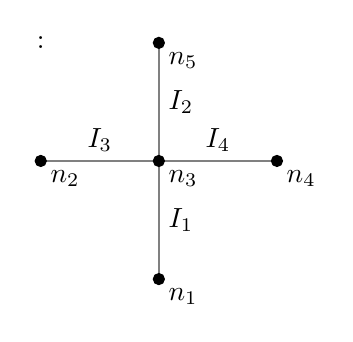
\begin{tikzpicture}
		\draw[gray, thick] (1.5,0) -- (1.5,3);
		\draw[gray, thick] (0,1.5) -- (3,1.5);
		\filldraw[black] (1.5,0) circle (2pt) node[anchor=north west] {$n_{1}$};
		\filldraw[black] (0,1.5) circle (2pt) node[anchor=north west] {$n_{2}$};
		\filldraw[black] (3,1.5) circle (2pt) node[anchor=north west] {$n_{4}$};
		\filldraw[black] (1.5,3) circle (2pt) node[anchor=north west] {$n_{5}$};
		\filldraw[black] (1.5,1.5) circle (2pt) node[anchor=north west] {$n_{3}$};
		\node[anchor=west] at (1.5, 0.75) {$I_{1}$};
		\node[anchor=west] at (1.5, 2.25) {$I_{2}$};
		\node[anchor=south] at (0.75, 1.5) {$I_{3}$};
		\node[anchor=south] at (2.25, 1.5) {$I_{4}$};
		\node at (0,3) {$\graph$:};
	\end{tikzpicture}
	\caption{The unit cell of the graph $\graph$; embedded in $\reals^{2}$ and periodic in 2 dimensions. \label{fig:GraphODEDiagram}}
\end{figure}
$\graph$ is chosen because it's structure is identical to that of the effective singular-structure problem for the thin-structure problem discussed in \cref{Homogenisation}.
$\graph$ consists of 5 vertices $V=\mathset{v_{1},v_{2},v_{3},v_{4},v_{5}}$ and 4 edges $E = \mathset{e_{13}, e_{35}, e_{23}, e_{34}}$, and is embedded in $\reals^{2}$.
We identify each vertex with a point in $\reals^{2}$ (cf \sref{GraphPrelims})
\begin{align*}
	\mathbf{v}_{1} = \bracs{\half,0}, \mathbf{v}_{2} = \bracs{0,\half} 
	\mathbf{v}_{3} = \bracs{\half, \half}, 
	\mathbf{v}_{4} = \bracs{1,\half}, \mathbf{v}_{5} = \bracs{\half, 1},
\end{align*}
and identify the edges with intervals
\begin{align*}
	e_{13} = I_{1} = \left[0,\half\right], \quad e_{35} = I_{2} = \left[\half,1\right], \quad
	e_{23} = I_{3} = \left[0,\half\right], \quad e_{34} = I_{4} = \left[\half,1\right],
\end{align*}
where we adopt a single index for the intervals for later simplicity. 
Denote the solution to a particular ODE posed along an edge with interval $I_{j}$ as $u_{j}$, so that the solution on the whole graph can be given by its associated set of edge solutions $\mathset{u_{j}:I_{j}\rightarrow\compx}$. \newline

Throughout this section we will be looking at the spectrum of the scalar-divergence operator 
\begin{align*}
	\graphOp u = -\laplacian u,
\end{align*}
on a periodic graph (hence the effective problem for a thin-structure problem in a periodic domain).
We will work in the low-frequency framework, and shall take $\graph$ as the unit cell of the singular-structure.
Introducing the length-scale $N$ we let $\graph_{N}$ be the square domain formed from $N^{2}$ copies and translations of $\graph$ (schematically illustrated in \fref{GraphODENPeriodsDiagramA}).
We introduce a labelling system for each periodic cell (copy of $\graph$) using the location of the bottom-left (south-west) corner of the unit cell --- hence the cell with label $(x',y')$ is the cell that is contained in $[x',x'+1]\times[y',y'+1]$.
For a cell with label $\bracs{x',y'}$ we denote the vertices with $v_{x',y', k}$ and edges with $e_{x',y',kl}$\footnote{With $k,l\in\{1,...,5\}$ and $j\in\{1,...,4\}$.} and maintain the local numbering system of $\graph$ (illustrated in \fref{GraphODENPeriodsDiagramB}).
Hence the edges are identified with the intervals $I_{x',y',j}$:
\begin{align*}
	e_{x',y',13} = I_{x',y',1} = \left[y', y'+\half \right], &\quad e_{x',y',35} = I_{x',y',2} = \left[ y'+\half, y'+1 \right], \\
	e_{x',y',23} = I_{x',y',3} = \left[x', x'+\half \right], &\quad e_{x',y',34} = I_{x',y',4} = \left[ x'+\half, x'+1 \right],
\end{align*}
and we denote the solution along an edge associated with interval $I_{x',y',j}$ as $u_{x',y',j}$.
We also number the cells from $0$ through to $N^{2}-1$, along the $x$ then $y$ directions (which will be useful later, when we need to construct linear systems on $\graph_{N}$).
This construction of $\graph_{N}$ results in vertices \say{on top of} one another: in an $N=2$ for example, system the vertices $v_{0,0,4}$ and $v_{1,0,2}$ are both positioned at $\bracs{1,\half}$, and so we identify these vertices with each other.
Finally, we refer to the vertices that lie on any of the lines $x=0, x=N, y=0, y=N$ as \say{hanging vertices} or  and all other vertices are called \say{interior vertices}.
At the hanging vertices we impose the periodicity conditions, identifying the nodes at $x=0$ with those as $x=N$ and similarly for the $y$-direction.
The interior nodes will have boundary conditions imposed at them, which is determined by the scaling of the vertex and edge volumes, $\vVol$ and $\eVol$ according to \sref{AsymRegimes}.
Finally (in a slight abuse of notation) we let $\graph_{\infty}$ denote the singular-structure that occupies the whole of $\reals^{2}$, with unit cell $\graph$.
Note that the previous labelling convention for cell $\bracs{x',y'}$ are still applicable in this case.
\begin{figure}[h]
    \centering
    \subfigure[The arrangement of the peridoic cells in the domain. Each cell is a translated copy of $\graph$, and they are arranged in an $N\times N$ square. The labelling of the components of the unit cell is shown to the right. \label{fig:GraphODENPeriodsDiagramA}]{
        \centering
			\begin{tikzpicture}
				\draw[step=1.5,gray,very thin, dashed] (0,0) grid (6.0,6.0);
				\node at (0.75,0.75) {$0$};
				\node at (2.25,0.75) {$1$};
				\node at (3.75,0.75) {$...$};
				\node at (5.25,0.75) {$N-1$};
				\node at (0.75,2.25) {$N$};
				\node at (2.25,2.25) {$...$};
				\node at (5.25,2.25) {$2N-1$};
				\node at (0.75,3.75) {$\vdots$};
				\node at (5.25,3.75) {$\vdots$};
				\node at (0.75,5.25) {$(N-1)N$};
				\node at (2.25,5.25) {$...$};
				\node at (5.25,5.25) {$N^{2}-1$};
			\end{tikzpicture}
	}
	\quad
    \subfigure[Local labelling of nodes and solution pieces within a unit cell $(x',y')$ \label{fig:GraphODENPeriodsDiagramB}]{
        \centering
			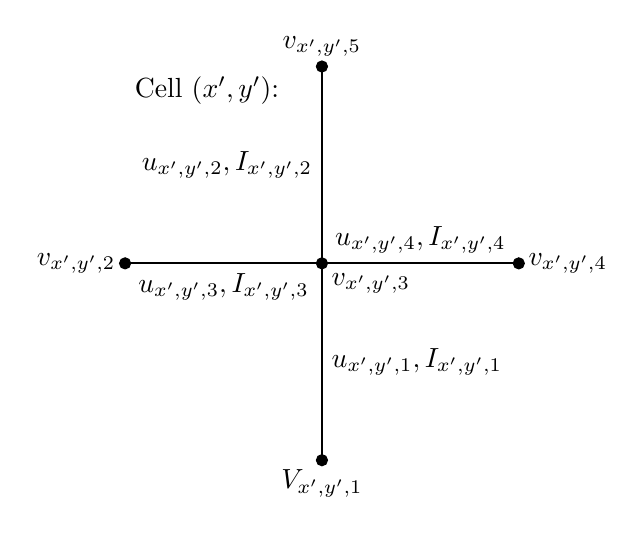
\begin{tikzpicture}
				\draw[black, thick] (0,-2.5) -- (0,2.5);
				\draw[black, thick] (-2.5,0) -- (2.5,0);
				\filldraw[black] (0,-2.5) circle (2pt) node[anchor=north] {$V_{x',y',1}$};
				\filldraw[black] (-2.5,0) circle (2pt) node[anchor=east] {$v_{x',y',2}$};
				\filldraw[black] (2.5,0) circle (2pt) node[anchor=west] {$v_{x',y',4}$};
				\filldraw[black] (0,2.5) circle (2pt) node[anchor=south] {$v_{x',y',5}$};
				\filldraw[black] (0,0) circle (2pt) node[anchor=north west] {$v_{x',y',3}$};
				\node[anchor=north] at (-1.25,0) {$u_{x',y',3}, I_{x',y',3}$};
				\node[anchor=south] at (1.25,0) {$u_{x',y',4}, I_{x',y',4}$};
				\node[anchor=west] at (0,-1.25) {$u_{x',y',1}, I_{x',y',1}$};
				\node[anchor=east] at (0,1.25) {$u_{x',y',2}, I_{x',y',2}$};
				\node[anchor=north west] at (-2.5,2.5) {Cell $(x',y')$:}; 
			\end{tikzpicture}
	}
	\caption{The domain $\graph_{N}$. Periodicity is imposed at the hanging vertices, and the conditions on the interior vertices are determined by the relative scaling of $\vVol$ and $\eVol$. \label{fig:GraphODENPeriodsDiagram}}
\end{figure} \newline

Finally, we include a brief analysis of the general eigenvalue-eigenfunction problem of the form
\begin{align*}
	-\left(\diff{x} + i\phi\right)^{2}v(x) &= \omega^{2} v(x), \quad x\in I \\
	\Leftrightarrow \ddiff{x}v + 2i\phi\diff{x}v - \phi^{2}v &= -\omega^{2}v,
\end{align*}
for some interval $I\subset\reals$ and function to be determined $v(x)$, with $\phi,\omega$ constants (hence the $2i\phi\diff{x} v$ term as opposed to the more general $\diff{x}\bracs{i\phi v} + i\phi\diff{x} v$).
The function $v=e^{\lambda x}$ solves this ODE, provided that
\begin{align*}
	\lambda^{2} + 2i\phi\lambda + (\omega^{2}-\phi^{2}) &= 0, \\
	\implies \lambda &= -i\phi \pm i\omega,
\end{align*}
and hence we obtain
\begin{align} \label{eq:EdgeSolutionForm}
	v(x) &= \emi{\phi x}\bracs{ c^{(1)}\ei{\omega x} + c^{(2)}\emi{\omega x} },
\end{align}
for constants $c^{(1)},c^{(2)}\in\compx$ which are determined by the boundary conditions at the endpoints of $I$ (at the vertices, for our cases).
This will be the form of the solutions along the edges $u_{j}$, and so we provide a corresponding subscript $c_{j}^{(1)},c_{j}^{(2)}\in\compx$ for the constants to be determined by the vertex conditions.

\section{Fast-Decaying Vertex Case}	\label{sec:GraphODE}
We begin with an example in the fast-decaying vertex case, which results in us obtaining continuity and (classical) Kirchhoff conditions at the interior nodes.
Using the Gelfand transform (\sref{GraphPrelims}) to analyse the spectrum of $\graphOp$ posed in $\graph_{\infty}$ requires introducing the quasi-momentum $\tho$ corresponding to the periodicity in the $x$-axis, and $\tht$ that in the $y$-axis. 
As the unit cell of $\graph_{\infty}$ is $\graph$ which is contained in the unit square, the range of both quasi-momentum is $\tho,\tht\in[-\pi,\pi)$.
We now look to analyse each of the operators $\graphOp^{\bracs{\tho,\tht}}$, and will obtain the spectrum of $\graphOp$ by taking the union of the spectra of $\graphOp^{\bracs{\tho,\tht}}$ over $\tho$ and $\tht$.
As the edges of $\graph$ are parallel to the co-ordinate axes, the operator $\graphOp^{\bracs{\tho,\tht}}$ reduces to the operation $-\left(\diff{x} + i\tho\right)^{2}$ on edges parallel to the $x$-axis and $-\left(\diff{x} + i\tht\right)^{2}$ on those parallel to the $y$-axis\footnote{In general the graph may have diagonal edges, and so the effect of the quasi-momentum on the operator along the edges is slightly more complex.}.
Working on $\graph$ means that we only have one interior vertex $v_{3}$, at which we have continuity and classical Kirchhoff conditions. 
Periodicity of the solution and first-derivative across $v_{1}\leftrightarrow v_{5}$ and $v_{2}\leftrightarrow v_{4}$ is also imposed. \newline

Compiling this information, we arrive at the system
\begin{subequations} \label{eq:GraphSystemFull}
\begin{align}
	-\left(\diff{x} + i\tho\right)^{2}u_{1}(x) &= \omega^{2} u_{1}(x),	&\quad x\in I_{1} \\
	-\left(\diff{x} + i\tho\right)^{2}u_{2}(x) &= \omega^{2} u_{2}(x),	&\quad x\in I_{2} \\
	-\left(\diff{x} + i\tht\right)^{2}u_{3}(x) &= \omega^{2} u_{3}(x),	&\quad x\in I_{3} \\
	-\left(\diff{x} + i\tht\right)^{2}u_{4}(x) &= \omega^{2} u_{4}(x),	&\quad x\in I_{4}
\end{align}
with the boundary conditions arising from continuity at $v_{3}$;
\begin{align}
	u_{1}\left(\half\right) &= u_{2}\left(\half\right), \label{eq:GraphODEc1}\\
	u_{1}\left(\half\right) &= u_{3}\left(\half\right), \\
	u_{3}\left(\half\right) &= u_{4}\left(\half\right), \label{eq:GraphODEc3}
\end{align}
from periodicity;
\begin{align}
	u_{1}(0) &= u_{2}(1), \\
	u_{3}(0) &= u_{4}(1), \\
	\left(\diff{x} + i\tho\right)u_{1}\eval{0} &= \left(\diff{x} + i\tho\right)u_{2}\eval{1}, \\
	\left(\diff{x} + i\tht\right)u_{3}\eval{0} &= \left(\diff{x} + i\tht\right)u_{4}\eval{1},
\end{align}
and from the classical Kirchhoff condition at $v_{3}$,
\begin{align}
	0 &= \sum_{j=1}^{4}\left(-1\right)^{j}\left(\diff{x} + i\theta_{\ceil{j/2}}\right)u_{j}\eval{\half}, \label{eq:GraphODEKirchhoffCond}
\end{align}
\end{subequations}
with $\ceil{x}$ denoting the ceiling function applied to $x$, which we use to give the Kirchhoff condition a succinct form.
Note also the factor of $\left(-1\right)^{j}$ in the Kirchhoff condition, accounting for the direction of the derivative into $v_{3}$.
Using the short analysis in this chapter's introduction, the edge solutions $u_{j}$ have the form of  \eref{EdgeSolutionForm},
\begin{align*}
	u_{j}(x) &= \emi{\theta_{\ceil{j/2}}x}\left(c_{j}^{(1)}\ei{\omega x} + c_{j}^{(2)}\emi{\omega x}, \right)
\end{align*}
for constant coefficients $c_{j}^{(k)}\in\compx$ ($k\in\{1,2\}$) to be determined by the boundary conditions \eref{GraphODEc1}-\eref{GraphODEKirchhoffCond}.
Determining these constants amounts to solving the linear system $A_{\infty}\bracs{\omega}\mathbf{c}=0$; where $\mathbf{c}$ the column vector of the coefficients (ordered by $j$ then the superscript), and $A_{\infty}$ the matrix
\begin{align}
	%A &=	
	\begin{pmatrix}
		\eiot{\omega}	&\emiot{\omega}	&-\eiot{\omega}	&-\emiot{\omega}	&0	&0	&0	&0	\\
		\eiot{\bracs{\omega-\tho}}	&\emiot{\bracs{\omega+\tho}}	&0	&0	&-\eiot{\bracs{\omega-\tht}}	&-\emiot{\bracs{\omega+\tht}}	&0	&0	\\
		0	&0	&0	&0	&\eiot{\omega}	&\emiot{\omega}	&-\eiot{\omega}	&-\emiot{\omega}	\\
		1	&1	&-\ei{\bracs{\omega-\tho}}	&-\emi{\bracs{\omega+\tho}}	&0	&0	&0	&0	\\
		0	&0	&0	&0	&1	&1	&-\ei{\bracs{\omega-\tht}}	&-\emi{\bracs{\omega+\tht}}	\\
		1	&-1	&-\ei{\bracs{\omega-\tho}}	&\emi{\bracs{\omega+\tho}}	&0	&0	&0	&0	\\
		0	&0	&0	&0	&1	&-1	&-\ei{\bracs{\omega-\tht}}	&\emi{\bracs{\omega+\tht}}\\
		-\eiot{\bracs{\omega-\tho}}	&\emiot{\bracs{\omega+\tho}}	&\eiot{\bracs{\omega-\tho}}	&-\emiot{\bracs{\omega+\tho}}	&-\eiot{\bracs{\omega-\tht}}	&\emiot{\bracs{\omega+\tht}}	&\eiot{\bracs{\omega-\tht}}	&-\emiot{\bracs{\omega+\tht}}	\\
	\end{pmatrix}
\end{align}
formed from the boundary condition equations.
Those $\omega$ that correspond to eigenfrequencies are those for which we have $\det\bracs{A_{\infty}}=0$, so that the vector $\mathbf{c}\neq\mathbf{0}$ and hence we obtain non-trivial solution $u$.
With some calculation it can be shown that this requires
\begin{align}
	\begin{split}
		0 = \sin\bracs{\omega}	
		[&-2\emi{\tho}\emi{\tht}e^{2i\omega} \\
		&+ \bracs{	\emi{\tho}e^{-2i\tht}  + e^{-2i\tho}\emi{\tht} + \emi{\tho} + \emi{\tht}	}\ei{\omega} \\
		&- 2\emi{\tho}\emi{\tht}	].	\\
	\end{split}
\end{align}
Note that the factor of $\sin\bracs{\omega}$ implies that $\omega=n\pi$ for $n\in\naturals$ is an eigenfrequency for all $\tho,\tht$. Otherwise, we can write the second factor in a more explicit form,
\begin{align} \label{eq:GraphODEOmSol2}
%	\omega &= n\pi, \quad n\in\naturals \mathrm{\: or \:}  \label{eq:GraphODEOmSol1}\\
%	\begin{split} \label{eq:GraphODEOmSol2}
%		e^{i\omega} = \recip{4}e^{i\tho}e^{i\tht} [
%			&\emi{\tho}e^{-2i\tht}  + e^{-2i\tho}\emi{\tht} + \emi{\tho} + \emi{\tht}  \\
%			&\pm \bracs{\emi{\tho}\emi{\tht}\left[\emi{\tho}+\emi{\tht}+4\right] +\emi{\tho} +\emi{\tht}}^{\half} \\
%			&\times\bracs{\emi{\tho}\emi{\tht}\left[\emi{\tho}+\emi{\tht}-4\right] +\emi{\tho} +\emi{\tht}}^{\half}
%		].
%	\end{split}
	\ei{\omega} &= \cos\bracs{\frac{\tho+\tht}{2}}\cos\bracs{\frac{\tho-\tht}{2}} \pm i\bracs{1-\cos^{2}\bracs{\frac{\tho+\tht}{2}}\cos^{2}\bracs{\frac{\tho-\tht}{2}}}^{\half}.
\end{align}
If a particular $\omega$ satisfies \eref{GraphODEOmSol2} (for given $\tho, \tht$), then $\omega+2n\pi$ also satisfies \eref{GraphODEOmSol2} for any $n\in\naturals$, and therefore the spectrum of the problem \eref{GraphSystemFull} can be fully described by only considering $\omega\in(0, 2\pi]$ and extending periodically.
Recognising real and imaginary parts of both sides of \eref{GraphODEOmSol2}, we can find explicit expressions for trigonometric functions of $\omega$:
\begin{subequations} \label{eq:ClassicalKirchhoffOmegaEquations}
\begin{align}
	\cos\bracs{\omega} &= \cos\bracs{\frac{\tho+\tht}{2}}\cos\bracs{\frac{\tho-\tht}{2}}, \label{eq:ClassKirchhoffOmEq1}\\
	\sin\bracs{\omega} &= \pm\bracs{1-\cos^{2}\bracs{\frac{\tho+\tht}{2}}\cos^{2}\bracs{\frac{\tho-\tht}{2}}}^{\half}. \label{eq:ClassKirchhoffOmEq2}
\end{align}
\end{subequations}
By use of the identity $\sin^{2}\phi + \cos^{2}\phi = 1$ it can be shown that $\omega$ satisfies \eref{ClassKirchhoffOmEq1} if and only if $\omega$ satisfies \eref{ClassKirchhoffOmEq2}, so it is sufficient to use only one of these equations to determine values of $\omega$.
As $\tho,\tht\in[-\pi,\pi)$ the right hand side of \eref{ClassKirchhoffOmEq1} attains every value in the interval $(-1,1]$ as $\tho$ and $\tht$ vary in this range; hence every $\omega\in(0,\pi)\cup(\pi,2\pi)$ will be a solution to this equation for some (not necessarily unique) pair of $(\tho,\tht)$.
Combined with the earlier deduction that $\omega=n\pi$ is an eigenfrequency for all values of $\tho,\tht$, this implies that the union over $\tho,\tht$ of all eigenfrequencies $\omega$ is the interval $(0,2\pi]$.
Hence by the $2\pi$-periodicity of the solutions for $\omega$, the spectrum of $\graphOp$ is the entire positive real line, $(0,\infty)$. \newline

Next we consider the sequence of (finite-frequency approximation) problems $\graphOp_{N}u = -\laplacian u$ for functions $u\in\lp{2}{\graph_{N}}$.
Let $\sigma_{N}$ denote the spectrum of $\graphOp_{N}$ for each $N\in\naturals$.
We can recycle the above analysis to determine $\sigma_{1}$, as by setting $\tho=\tht=0$ we obtain the setup for the $N=1$ problem.
This provides the spectrum $\sigma_{1} = \mathset{n\pi \text{ }\vert\text{ } n\in\naturals}$.
For the other cases, we systematically associate each $1\times1$ cell of $\graph_{N}$ with 8 boundary conditions.
A cell $\bracs{x',y'}$ provides 3 equations from continuity at the vertex $v_{x',y',3}$ and 1 equation from the Kirchhoff condition at the same vertex, which involve only arbitrary constants of solutions $u_{x',y',j}$ (that is, only edge solutions that belong to the cell itself).
The other 4 conditions relate to other neighbouring cells at the edge vertices of the cell - we associate the conditions including the neighbouring cells to the \say{left} and \say{below}.
That is, we associate the matching conditions (continuity of solution and first derivative) at $v_{x',y',2}\leftrightarrow v_{x'-1,y',4}$ and $v_{x',y',1}\leftrightarrow v_{x',y'-1,5}$, replacing these with the appropriate periodic conditions in the event that $x'=0$ or $y'=0$.
This gives us the $8N^{2}\times8N^{2}$ system $A_{N}\bracs{\omega}\mathbf{c}_{N} = \mathbf{0}$ where $\mathbf{c}_{N}$ is the vector of arbitrary constants of the edge solutions (now ordered by cell label, then $j$, then superscript) and $A_{N}$ is the matrix for the linear system of equations, which has sparsity pattern as shown in \fref{ANSparsityPattern} thanks to the method of associating boundary conditions with each cell.
$\det\bracs{A_{N}\bracs{\omega}}$ is $2\pi$-periodic in $\omega$ when $N$ is odd, and $\pi$-periodic when $N$ is even (one can deduce this from the form of the boundary conditions and the way $\omega$ appears in them).
Additionally, the determinant is entirely imaginary for odd $N$, and entirely real for even $N$.
Computations examining $\det\bracs{A_{N}\bracs{\omega}}$ imply that $\omega=n\pi$ is a root of this quantity for every $N, n\in\naturals$; and furthermore each $N$ produces $2N$ other roots for $\omega\in\bracs{0,2\pi}\setminus\mathset{\pi}$, however this is hard to verify analytically due to the size of $A_{N}$.
However it can be seen that the number of solutions for $\omega$ is increasing with $N$; and these are becoming increasing \say{dense} along the real line, as we expect due to our knowledge of the full-space problem.
Some examples of $\det\bracs{A_{N}\bracs{\omega}}$ are shown in \fref{FastDecayDets}.
\begin{figure}[b!]
    \centering
    \subfigure[Sparsity pattern of the matrix $A_{N}$, for $N=4$. Entries that are not in the diagonal ``blocks" correspond to conditions that involve multiple unit cells.\label{fig:ANSparsityPattern}]{
    	\centering
        \includegraphics[scale=0.6]{./Images/MatrixSparsityPattern.png}
	}
	\quad
    \subfigure[The quantity $\det\bracs{A_{N}\bracs{\omega}}$ over the range $\bracs{0,2\pi}$, for $N=1,2,3,4$. Periodicity of the determinant can be seen. Note that values are normalised for each $N$ to allow for visualisation. \label{fig:FastDecayDets}]{
        \centering
		\includegraphics[scale=0.6]{./Images/MatrixDetsFastDecay.png}
	}
	\caption{The sparsity pattern of the matrix $A_{N}$ (left) and the behaviour of it's determinant as a function of $\omega$ (right).}
\end{figure}

\section{Borderline Case (Non-Classical Kirchhoff Condition)} \label{sec:Graph2DNonClassicalKirchhoff}
Following the conclusion of \sref{GraphODE}, we now explore the borderline vertex-scaling case, and illustrate the concept of "spectral band gaps".
Again we first consider the domain $\graph_{\infty}$, and seek the spectrum of the operator $\graphOp$; only this time consider ourselves in the borderline case and impose a non-classical Kirchhoff condition at the interior vertices.
We introduce the quasi-momentum $\tho,\tht\in[-\pi,\pi)$ and family of operators $\graphOp^{\bracs{\tho,\tht}}$, and analyse a problem posed on (the unit cell) $\graph$.
We obtain a system analogous to \eref{GraphSystemFull} but with the Kirchhoff condition at $v_{3}$ replaced with the \say{non-classical Kirchhoff} condition
\begin{align*}
	\alpha\omega^{2}u\bracs{\mathbf{v}_{3}} = \sum_{j=1}^{4}\left(-1\right)^{j}\left(\diff{x} + i\theta_{\ceil{j/2}}\right)u_{j}\eval{\half}, %\label{eq:GraphODENonClassicalKirchhoffCond}
\end{align*}
where $u\bracs{\mathbf{v}_{3}}$ is the value of the solution at the central vertex (which exists due to the condition of continuity at $v_{3}$) and $\alpha$ a constant which is related to $\vVol$.
Again we can express the resulting system as a matrix equation $A_{\infty}\bracs{\omega}\mathbf{c}=\mathbf{0}$\footnote{One can make a choice of $u\bracs{\mathbf{v}_3}$ as any of the edge solutions $u_{j}$ evaluated at $\half$.}.
Again we seek those $\omega$ which solve $\det\bracs{A_{\infty}\bracs{\omega}}=0$, which can be shown to be those $\omega$ which satisfy the equation
\begin{align*}
	0 &= \half i\alpha\omega\bracs{e^{2i\omega}-1}\bracs{ \frac{\alpha\omega}{4}\sin\bracs{\omega} + \cos\bracs{\omega} - \cos\bracs{\frac{\tho-\tht}{2}}\cos\bracs{\frac{\tho+\tht}{2}} }.
\end{align*}
This means that $\omega=n\pi$ for any $n\in\naturals_{0}$ is a solution, due to the factor of $e^{2i\omega}-1$.
Other values for $\omega$ do not have a closed form and must be determined numerically from the equation
\begin{align}
	\frac{\alpha\omega}{4}\sin\bracs{\omega} + \cos\bracs{\omega} &= \cos\bracs{\frac{\tho-\tht}{2}}\cos\bracs{\frac{\tho+\tht}{2}}, \label{eq:GraphNonClassicalTransendental}
\end{align}
however we can make some deductions about the spectrum of $\graphOp$ analytically.
For ease of reference we denote the left hand side of \eref{GraphNonClassicalTransendental} by the function
\begin{align*}
	\trfn\bracs{\omega}:(0,\infty)&\rightarrow\reals, \\
	\omega &\mapsto \frac{\alpha\omega}{4}\sin\bracs{\omega} + \cos\bracs{\omega},
\end{align*}
and the right hand side by
\begin{align*}
	\Psi\bracs{\tho,\tht}:[-\pi,\pi)^{2}&\rightarrow\reals, \\
	\bracs{\tho,\tht}&\mapsto \cos\bracs{\frac{\tho-\tht}{2}}\cos\bracs{\frac{\tho+\tht}{2}}.
\end{align*}
$\Psi$ is continuous in both it's variables, and is bounded between (and attains) $-1$ and $1$ hence achieves every value in the interval $[-1, 1]$.
For a given $\bracs{\tho,\tht}$, \eref{GraphNonClassicalTransendental} has constant right-hand side and is equivalent to seeking a level set of $\trfn$.
Hence the spectrum (the union over all $\tho,\tht$ of eigenfrequencies $\omega$) are those $\omega$ for which $\trfn\bracs{\omega}$ lies in the image of $\Psi$, namely those $\omega$ for which
\begin{align} \label{eq:OmegaCriterion}
	-1 \leq \frac{\alpha\omega}{4}\sin\bracs{\omega} + \cos\bracs{\omega} &\leq 1.
\end{align}
One can visualise the function $\trfn$ in \fref{NonClassicalKirchhoffTransendentalLHS}, and the corresponding spectral values that are obtained in \fref{SpectralBands2dGraphNonClassicalKirchhoff}.
As can be seen, the spectral values appear to form a disjoint set of intervals, the \say{spectral bands} or simply \say{bands}.
\begin{figure}[t!]
    \centering
    \subfigure[The function $\trfn$ plotted for $0\leq\omega\leq 6\pi$. The black lines are positioned at $-1$ and 1 on the y-axis, so whenever the red line lies between the black lines the corresponding $\omega$ is an eigenfrequency. One can see visually that the eigenfrequencies are separated into disjoint intervals. \label{fig:NonClassicalKirchhoffTransendentalLHS}]{
        \centering
        \includegraphics[scale=0.42]{./Images/NonClassicalKirchhoffTransendentalLHS.png}
	}
	\quad
    \subfigure[Illustration of the spectral bands in $\omega$ that arise from the 2D graph problem with a non-classical Kirchhoff condition at the central vertex. Blue crosses correspond to eigenfrequencies at $\omega=n\pi$ for $n\in\naturals_{0}$. Note that the length of successive bands is decreasing, and each $n\pi$ is the right-endpoint of a band.\label{fig:SpectralBands2dGraphNonClassicalKirchhoff}]{
        \centering
		\includegraphics[scale=0.42]{./Images/SpectralBandsNonClassicalKirchhoff2DGraph.png}
	}
	\caption{The relation between the function $\trfn$ and the spectral values $\omega$. \label{fig:NonClassicalKirchhoffStuff}}
\end{figure} \newline

Going further than visual inspection, it can be proved that the operator $\graphOp$ has a genuine band-gap spectrum - a union of \say{(spectral) bands} $I_{n}$ for $n\in\naturals$.
This follows from some analysis of $\trfn$, for which we need the following result:
\begin{lemma}[Critical Points of $\trfn$] \label{lem:CritPtsOmega}
	Let $n\in\naturals$. Then $\trfn$ has at most one critical point in the interval $((n-1)\pi, n\pi)$. \newline
	Equivalently, $\trfn^{\prime}$ has at most one root in the interval $((n-1)\pi, n\pi)$.
\end{lemma}
\begin{proof}
	Note that
	\begin{align} \label{eq:OmegaPrimeEqn}
		\trfn^{\prime}\bracs{\omega} &= \frac{\alpha\omega}{4}\cos\bracs{\omega} + \bracs{\frac{\alpha}{4} - 1}\sin\bracs{\omega}.
	\end{align}
	In the case $\alpha=4$, \eref{OmegaPrimeEqn} reduces to $\trfn^{\prime}\bracs{\omega} = \omega\cos\bracs{\omega}$. 
	As $\omega>0$, roots can only occur when $\cos\bracs{\omega}=0$, which occurs precisely once for $\omega\in((n-1)\pi, n\pi)$ - at $\omega=\bracs{n-\half}\pi$. \newline
	Otherwise we express $\trfn^{\prime}$ using a single trigonometric function,
	\begin{align} \label{eq:OmegaPrimeAlt}
		\trfn^{\prime}\bracs{\omega} &= \recip{4}\bracs{\alpha^{2}\bracs{\omega^{2}+1}-8\alpha+16}^{\half}\sin\bracs{\omega + \tan^{-1}\bracs{\frac{\alpha\omega}{\alpha-4}}}.
	\end{align}
	Now
	\begin{align*}
		\alpha^{2}\bracs{\omega^{2}+1}-8\alpha+16 &\leq 0, \\
		\Leftrightarrow \omega^{2} &\leq -\recip{\alpha^{2}}\bracs{\alpha-4}^{2},
	\end{align*}
	which posthumously justifies the use of the square-root, and also implies that $\trfn^{\prime}=0$ only when the sine factor is equal to zero.
	Now note that $\tan^{-1}\bracs{\abs{\frac{\alpha}{\alpha-4}}\omega}$ is bounded below by $0$ and above by $\frac{\pi}{2}$.
	Hence, in the case when $\alpha>4$, $\abs{\frac{\alpha}{\alpha-4}}=\frac{\alpha}{\alpha-4}$ and so
	\begin{align*}
		(n-1)\pi &< \omega + \tan^{-1}\bracs{\abs{\frac{\alpha}{\alpha-4}}\omega} < \bracs{n+\half}\pi, \\
	\end{align*}
	and over the interval $\bracs{(n-1)\pi, \bracs{n+\half}\pi}$, the sine function has precisely one root. Hence $\trfn^{\prime}$ as at most one root for $\omega\in((n-1)\pi,n\pi)$, in this case.
	In the case $\alpha<4$, we simply note that $\tan^{-1}\bracs{\frac{\alpha\omega}{\alpha-4}}=-\tan^{-1}\bracs{\abs{\frac{\alpha}{\alpha-4}}\omega}$, hence
	\begin{align*}
		\bracs{n-1-\half}\pi &< \omega - \tan^{-1}\bracs{\abs{\frac{\alpha}{\alpha-4}}\omega} < n\pi, \\
	\end{align*}
	and over the interval $\bracs{\bracs{n-1-\half}\pi, n\pi}$ the sine function again has precisely one root; hence $\trfn^{\prime}$ has at most one root in $\omega\in((n-1)\pi,n\pi)$, which concludes all cases and provides the result.
\end{proof}

Knowledge of the critical points of $\trfn$ allows us to deduce that the spectrum is a union of intervals (justifying the use of the term \say{band}), with each interval containing exactly one multiple of $\pi$ at it's right endpoint. 
\begin{prop}[Spectral Bands, $n\geq2$] \label{prp:SpecBandsn2}
	For each $n\geq2$ with $n\in\naturals$, there exists a $c_{n}\in((n-1)\pi,n\pi)$ such that 
	\begin{enumerate}
		\item $\abs{\trfn}\leq1$ on the interval $I_{n}:=[c_{n}, n\pi]$, 
		\item $\abs{\trfn}>1$ on the interval $((n-1)\pi, c_{n})$, and
		\item $I_{n}$ is the largest interval containing $n\pi$ on which $\abs{\trfn}\leq1$.
	\end{enumerate}
\end{prop}
\begin{proof}
	We first assume that $n$ is even.
	Then by direct computation we can find that
	\begin{align*}
		\trfn\bracs{(n-1)\pi} = -1, &\quad \trfn\bracs{n\pi} = 1, \\
		\trfn^{\prime}\bracs{(n-1)\pi} <0, &\quad \trfn^{\prime}\bracs{n\pi} >0.
	\end{align*}
	As $\trfn^{\prime}$ is continuous and changes sign over $[(n-1)\pi, n\pi]$, it has at least one root (by the Intermediate Value Theorem) in the interior of this interval.
	Combined with the result from \lref{CritPtsOmega}, it has precisely one root in this interval.
	Hence $\trfn$ has exactly one critical point in this interval.
	Furthermore, as $\trfn^{\prime}\bracs{(n-1)\pi}<0$ there exists some $\delta>0$ such that $\trfn\bracs{\omega}<\trfn\bracs{(n-1)\pi}=-1$ for all $\omega\in((n-1)\pi, (n-1)\pi+\delta)$.
	But $\trfn$ is continuous and $\trfn\bracs{n\pi}=1$, and thus $\trfn$ must cross $-1$ again, at a point $c_{n}\in[(n-1)\pi+\delta, n\pi)$.
	Hence over the interval $((n-1)\pi,c_{n})$ we have $\trfn<-1$, with $\trfn=-1$ at $(n-1)\pi$ and $c_{n}$ (in particular, $\abs{\trfn}>1$).
	This implies that $\trfn$ has a critical point in this interval, which by the above reasoning is it's only critical point in $((n-1)\pi, n\pi)$.
	Hence the choice of $c_{n}$ is unique, and furthermore $\trfn\leq1$ on $(c_{n},n\pi)$ (were this not the case, this would imply $\trfn$ had additional critical points to allow for \say{turning back} on itself), so we have that $-1\leq\trfn\leq1$ on $I_{n}:=[c_{n}, n\pi]$.
	It remains to show that $I_{n}$ is the largest such interval containing $n\pi$; and by the argument just concluded cannot extend the left endpoint of $I_{n}$.
	As for the right endpoint, $n\pi$ itself; we note that $\trfn^{\prime}\bracs{n\pi}>0$ here and $\trfn\bracs{n\pi} = 1$, hence there exists some $\epsilon>0$ such that $\trfn>1$ on $(n\pi, n\pi+\epsilon)$.
	Hence, we cannot extend the right endpoint either, and the result holds. \newline
	For the case when $n$ is odd, an analogous argument holds, with reversed inequalities and similar reasoning.
\end{proof}

The case when $n=1$ is separate because this case requires an understanding of the behaviour of $\trfn$ near 0. 
For the analysis that follows it is convenient to temporarily extend the domain of $\trfn$ to the other side of 0, say to $(-\half, \infty)$, so that we can use arguments based on properties of $\trfn$ and it's derivatives at 0 (without formally introducing one-sided derivatives and the like).
\begin{prop}[Spectral Band, $n=1$] \label{prp:SpecBandsn1}
	For consistency, we use similar notation to \pref{SpecBandsn2}.
	\begin{enumerate}
		\item If $\alpha\leq2$, then the interval $I_{1}:=(0,\pi]$ is the largest interval which contains $\pi$ and on which $\abs{\trfn}\leq1$.
		\item If $\alpha>2$, there exists a $c_{1}\in(0,\pi)$ such that the interval $I_{1}:=[c_{1},\pi]$ is the largest interval which contains $\pi$ and on which $\abs{\trfn}\leq1$, and $\abs{\trfn}>1$ on $(0,c_{1})$.
	\end{enumerate}
\end{prop}
Note that the difference between cases is very subtle, namely that if $\alpha\leq2$ then $c_{1}=0$ and $I_{n}$ is half-open on the left; otherwise the conclusion is the same as in \pref{SpecBandsn2}.
\begin{proof}
	We begin by evaluating $\trfn$ at $\pi$ and 0:
	\begin{align*}
		\trfn\bracs{\pi} = -1,		&\quad \trfn^{\prime}\bracs{\pi} < 0, \\
		\trfn\bracs{0} = 1,		&\quad \trfn^{\prime}\bracs{0} = 0.
	\end{align*}
	Like \pref{SpecBandsn2}, the properties of $\trfn$ and $\trfn^{\prime}$ at $\pi$ lead to the conclusion that any interval which we seek must have right endpoint $\pi$.
	Unlike the $n\geq2$ cases, $\trfn^{\prime}\bracs{0}=0$ so we cannot repeat the argument of \pref{SpecBandsn2} as we required knowledge of how the derivative behaved, which informed behaviour of $\trfn$.
	Instead, we turn to the second derivative of $\trfn$ at 0, which is
	\begin{align*}
		\trfn^{\prime\prime}\bracs{0} &= \frac{\alpha}{2}-1.
	\end{align*} \newline
	\underline{Case $\alpha<2$}: In this case $\trfn^{\prime\prime}<0$ and so $\trfn$ has a local maximum at 0.
	Hence there exists an $\epsilon>0$ such that $\trfn<1$ on $(-\epsilon, \epsilon)$, in particular $\Omega<1$ on $(0, \epsilon)$.
	We now establish that $\trfn<1$ on all of $(0,\pi)$ by contradiction: if there existed a $d\in(0,\pi)$ where $\trfn>1$, $\trfn$ must have a critical point between $(0,d)$ (to \say{turn around} from the maximum at 0), and must also intersect $1$ at some $d_{-}\in(\epsilon,d)$. 
	However continuity of $\trfn$ between $d$ and $\pi$ implies that $\trfn$ intersects $1$ again at $d_{+}\in(d, \pi)$.
	Hence we have $d_{-} <d < d_{+}$ and also $\trfn\bracs{d_{-}} < \trfn\bracs{d} > \trfn\bracs{d_{+}}$ which implies the existence of a second critical point in $(d_{-},d_{+})$, contradicting \lref{CritPtsOmega} and giving us that $\trfn<1$ on all of $(0,\pi)$.
	We can also establish that $\trfn>-1$ on all of $(0,\pi)$: if if there existed a $d\in(0,\pi)$ where $\trfn<-1$, there exists a $d_{-}\in(0,d)$ where $\trfn\bracs{d_{-}}=-1$.
	However $\trfn\bracs{\pi}=-1$ so $\trfn$ has a critical point in the interval $(d_{-},\pi)$, because $\trfn\bracs{d_{-}}>\trfn\bracs{d}<\trfn\bracs{\pi}$ this is a local minimum.
	Without loss of generality, we can say that the local minimum occurs at $d$ (simply by changing labels of points).
	Now there exists a $\delta>0$ such that $\trfn^{\prime}>0$ on $(d,d+\delta)$ as $d$ is a local minimum; but $\trfn^{\prime}\bracs{\pi}<0$ so by continuity of $\trfn^{\prime}$ it has a root in $(d, \pi)$, thus requiring existence of two roots of $\trfn^{\prime}$ in $(0,\pi)$ contradicting \lref{CritPtsOmega}.
	Hence we have that $\abs{\trfn}<1$ on $(0,\pi)$, combined with $\trfn\bracs{\pi}=-1$ we have found that the spectral band $I_{1}=(0,\pi]$. \newline
	\underline{Case $\alpha>2$}: In this case $\trfn^{\prime\prime}>0$ and so $\trfn$ has a local minimum at 0.
	Hence there exists an $\epsilon>0$ such that $\trfn>1$ on $(-\epsilon, \epsilon)$, in particular $\trfn>1$ on $(0, \epsilon)$.
	Continuity of $\trfn$ then implies that there exists a $c_{1}\in(\epsilon,\pi)$ such that $\trfn\bracs{c_{1}}=1$.
	This also means that $\trfn$ must have a local maximum between $(0,c_{1})$, which is it's only critical point in $(0,\pi)$ by \lref{CritPtsOmega}.
	Thus we can establish that $-1\leq\trfn\leq1$ on $[c_{1}, \pi]$, as if this is not the case a second critical point for $\trfn$ must exist (see the argument in \pref{SpecBandsn2}) and that $\abs{\trfn}>1$ on $(0,c_{1})$.
	Hence $I_{1}=[c_{1},\pi]$ for $c_{1}\in(0,\pi)$. \newline
	\underline{Case $\alpha=2$}: Although the conclusion for this case is the same as that for the $\alpha<2$ case, different reasoning is required as in this case $\trfn^{\prime\prime}\bracs{0}=0=\trfn^{\prime\prime\prime}\bracs{0}$.
	We do find that $\trfn^{(4)}\bracs{0}<0$, which implies that $\trfn^{\prime\prime}$ has a local maximum at 0.
	Hence there exists an $\epsilon>0$ such that $\trfn^{\prime\prime}\bracs{\omega}<\trfn^{\prime\prime}\bracs{0}=0$ for all $\omega\in(-\epsilon,\epsilon)$.
	Now applying the Mean Value Theorem to $\trfn^{\prime}$ between $(-\epsilon,0)$, we find that there exists some $d\in(-\epsilon,0)$ such that $\trfn^{\prime\prime}\bracs{d}=\recip{\epsilon}\trfn^{\prime}\bracs{\epsilon}$.
	But $d\in(-\epsilon,0)$ and $\epsilon>0$ hence $\trfn^{\prime}\bracs{\epsilon}<0$.
	$\trfn^{\prime}$ is also an odd function, so $\trfn^{\prime}\bracs{-\epsilon}<0$ and hence
	\begin{align*}
		\trfn^{\prime}\bracs{-\epsilon} <0 <\trfn^{\prime}\bracs{\epsilon}.
	\end{align*}
	This also holds for any positive $\epsilon^{*}<\epsilon$ (the Mean Value Theorem is applied on $(-\epsilon^{*},0)$ instead); thus $\trfn$ has a point of inflection at 0, and because $\trfn^{\prime}<0$ on $(0,\epsilon)$, we have that there exists some $\delta>0$ such that $\trfn<1$ on $(0,\delta)$.
	We then revert to the previous analysis of the critical points to deduce that $\abs{\trfn}<1$ on all of $(0,\pi)$, and hence obtain the result.
\end{proof}
\Pref{SpecBandsn2} and \pref{SpecBandsn1} show that the spectral bands are all intervals, and a bijection exists from $\naturals$ to the set of spectral bands $\left\{I_{n} \text{ }\vert\text{ } n\pi\in I_{n}\right\}$.
In addition the spectral bands are disjoint; the $n^{\mathrm{th}}$ band terminates at $n\pi$, and all bands are closed intervals, unless $\alpha\leq2$ in which case the $n=1$ band is open on the left with left endpoint 0.
This is an important characteristic of the spectrum which we will revisit when we look to take a numerical approach at the corresponding thin-structure problem in \cref{Homogenisation}.

\section{Summary} \label{sec:GraphSummary}
The problems we have considered in this chapter demonstrate how the theory of \sref{GraphPrelims} and \sref{AsymRegimes} can be applied to singular-structures, to produce information about the spectrum of the operator we are concerned with.
The concept of a band-gap spectrum is important to an application of this theory in the context of PCFs, as a PCF is only useful if it can trap light in the core due to the presence of band-gaps!
The analysis thus performed is both much simpler than the methods associated with its multi-dimensional counterparts, most of which are numerical schemes which we will consider in \cref{Homogenisation}. \newline

This being said, the systems in this chapter are only simple examples of wider-reaching theory.
Without much effort it is possible to consider some of the generalisations to these systems:
\begin{itemize}
	\item Using a structure with edges parallel to the co-ordinate axes simplifies the analysis of the problem (particularly concerning determining the actions of the parametrised operators) however in doing so we also neglect the effect of the structure geometry.
	Introducing diagonal edges into a singular structure can lead to the opening of band-gaps in the fast-vertex scaling cases, and it is not hard to envisage graphs which not \say{centrally connected} or are even cyclic (like the honeycomb structure in \fref{PCFDiagram}).
	This is important for application to the design of optical fibres - fabrication techniques have greatly improved since the first optical fibres and so open up the possibility to explore more exotic geometric structure.
	\item The problem presented thus far has been a scalar-divergence equation, however an application to a physical system will require a formulation in terms of vector-valued functions on graphs.
	Whilst the idea of switching to a vector-valued function is not audacious, the effects this will have on the analysis of the systems may be more concerning.
	Vector-valued functions are almost always harder to work with than their scalar counterparts, and often result in the need to solve for the components in a coupled system of equations.
	There is also the need to investigate how to properly construct the singular-structure operator from the thin-structure operator we wish to approximate.
	This being said, with the additional complexity may come the possibility of unexplored effects which do not manifest in the scalar-case.
	\item A physical model for propagation also requires a time dependence, and hence a time derivative should appear in the operator.
	Whilst the effect of this is not fully understood, we can speculate on what it may mean for the singular-structure problem and previous analysis.
	The presence of a time-derivative immediately implies that the reduction to an ODE on the graph edges will no longer happen, as at the least the edge solutions will have to acknowledge the time-variation too.
	This will necessitate solution of a PDE on the edges, with the variables being the spatial direction along the edge and time.
	Whilst such PDEs are not unapproachable, in general less is understood about the solution to PDEs than ODEs.
	Perhaps a more effective approach may be to trial an ansatz for the solution to the system, such as a Bloch-wave $e^{i\bracs{\mathbf{k}\cdot\mathbf{x}-\omega t}}$, which reduces the original system of equations to a set of coupled time-independent equations; although with this assumption again comes the potential to exclude certain effects that time-dependence may induce on the spectrum.
\end{itemize}
A combination of these considerations will need to be considered for a PCF model, as we will see in \cref{WorkDirection}.